%! Author = melek
%! Date = 9.06.2022

% Preamble
\documentclass[11pt]{article}

% Packages
\usepackage{amsmath}
\DeclareMathOperator*{\argmax}{argmax}

\usepackage{graphicx}
\usepackage{amssymb}
\usepackage{bm}

\graphicspath{ {../images/} }


% Document
\begin{document}

    \maketitle
    \setcounter{section}{6}


    \section{Exercises}

    \subsection{Question}

    In Chapter 6 we noted that the Monte Carlo error can be written as the sum of TD errors (6.6) if the value estimates don’t change from step to step.
    Show that the n-step error used in (7.2) can also be written as a sum TD errors (again if the value estimates don’t change) generalizing the earlier result.

    \subsection*{Answer}

    Value estimates are assumed not to change thus we can omit value estimate subscripts such that $ V_t(S_t) = V_{t+1}(S_t)$.

    n-step TD Error used in 7.2  is:
    \newline
    $G_{t:t+n} - V(S_t) = R_{t+1} + \gamma G_{t+1:t+n} - V(S_t) $
    \newline
    $G_{t:t+n} - V(S_t) = R_{t+1} + \gamma V(S_{t+1}) - V(S_t) + \gamma G_{t+1:t+n} - \gamma V(S_{t+1}) $
    \newline
    $G_{t:t+n} - V(S_t) = \delta_t + \gamma ( G_{t+1:t+n} - V(S_{t+1}) ) $
    \newline
    $G_{t:t+n} - V(S_t) = \delta_t + \gamma \delta_{t+1} + \gamma^2 ( G_{t+2:t+n} - V(S_{t+2}) ) $
    \newline
    $G_{t:t+n} - V(S_t) = \sum_{k=t}^{t+n-1} \gamma^{k-t} \delta_k  $

    \subsection{Question}

    (programming) With an n-step method, the value estimates do change from step to step, so an algorithm that used the sum of TD errors (see previous exercise) in place of the error in (7.2) would actually be a slightly different algorithm.
    Would it be a better algorithm or a worse one?
    Devise and program a small experiment to answer this question empirically.

    \subsection*{Answer}

    The chart above shows regular n-step TD with different n parameters.
    The chart below shows the same configuration with unchanged value functions.
    Value function updates are applied only after an episode terminates.

    Using sum of TD errors as in place of the error in 7.2 performs worse in all n and $\alpha$ values.

    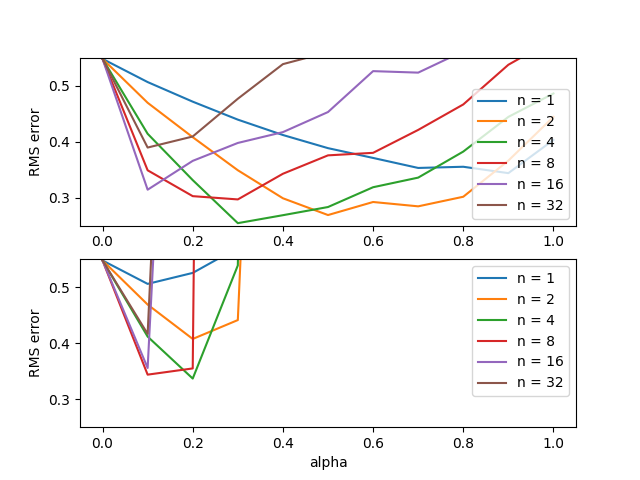
\includegraphics[scale=1]{figure_7_2}

    \subsection{Question}

    Why do you think a larger random walk task (19 states instead of 5) was used in the examples of this chapter?
    Would a smaller walk have shifted the advantage to a different value of n?
    How about the change in left-side outcome from 0 to -1 made in the larger walk?
    Do you think that made any difference in the best value of n?

    \subsection*{Answer}

    If n-step size is close to or bigger than the average number steps to complete an episode then the algorithm approaches to MC which involves variance.
    Using 19 states increases average number of steps to complete an episode thus helps to show how n-step size effects the algorithm.

    If number of states was 5, optimum n-step size would be smaller.
    An empiric study shows that if return value -1 is used with 5 states, most optimum n value would be 1.

    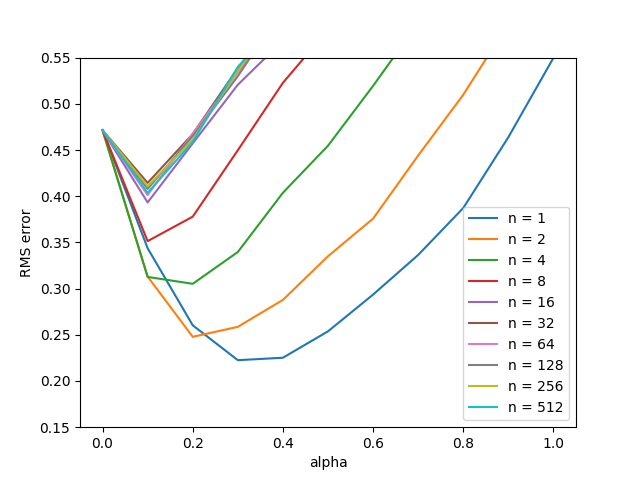
\includegraphics[scale=0.4]{figure_7_3_5states_ret-1}

    Randomwalk with 5 states and reward of 0 on the left, results are found to be different from the -1 case.
    We can interpolate and conclude that changing the return value may affect the result.

    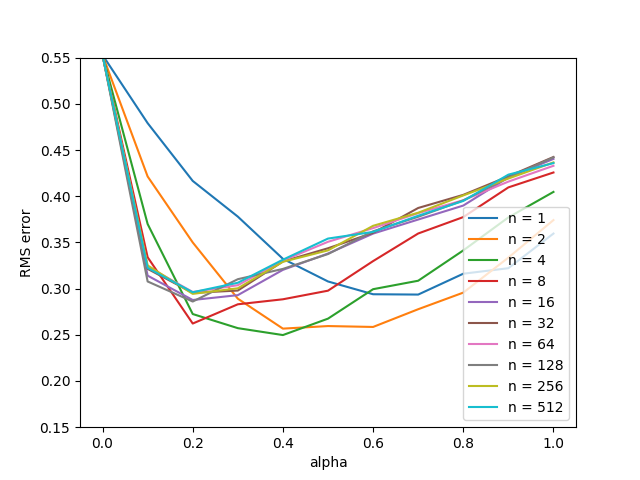
\includegraphics[scale=0.4]{figure_7_3_5states_ret0}

    \subsection{Question}

    Prove that the n-step return of Sarsa (7.4) can be written exactly in terms of a novel TD error.

    \subsection*{Answer}

    Given expression:
    \newline
    $ G_{t:t+n} = Q_{t-1}(S_t , A_t) + \sum_{ k=t}^{\min(t+n, T) - 1} \gamma^{k-t} [R_{k+1} + \gamma Q_{k}(S_{k+1} , A_{k+1}) - Q_{k-1}(S_{k} , A_{k}) ]  $
    \newline

    Can be expanded for n:
    \newline
    $ G_{t:t+n} = Q_{t-1}(S_t , A_t) + \gamma^{0} [R_{t+1} + \gamma Q_{t}\quad(S_{t+1} , A_{t+1}) - Q_{t-1}(S_{t} , A_{t}) ] $

    $  \qquad\qquad\qquad\qquad\  + \gamma^{1} [R_{t+2} + \gamma Q_{t+1}(S_{t+2} , A_{t+2}) - Q_{t}\ \ (S_{t+1} , A_{t+1}) ] $

    $  \qquad\qquad\qquad\qquad\  + \gamma^{2} [R_{t+3} + \gamma Q_{t+2}(S_{t+3} , A_{t+3}) - Q_{t+1}(S_{t+2} , A_{t+2}) ] $

    $ \dots $

     $  \qquad\qquad\qquad\qquad\  + \gamma^{n-1} [R_{t+n} + \gamma Q_{t+n-1}(S_{t+n} , A_{t+n}) - Q_{t+n-2}(S_{t+n-2} , A_{t+n-2}) ] $

    $\gamma$ distributed:
     \newline
    $ G_{t:t+n} = Q_{t-1}(S_t , A_t) + \quad R_{t+1} + \gamma Q_{t}\quad(S_{t+1} , A_{t+1}) - Q_{t-1}(S_{t} , A_{t})  $

    $  \qquad\qquad\qquad\qquad\  + \gamma \ R_{t+2} + \gamma^2 Q_{t+1}(S_{t+2} , A_{t+2}) - \gamma Q_{t}(S_{t+1} , A_{t+1}) ] $

    $  \qquad\qquad\qquad\qquad\  + \gamma^{2} R_{t+3} + \gamma^{3} Q_{t+2}(S_{t+3} , A_{t+3}) - \gamma^{2} Q_{t+1}(S_{t+2} , A_{t+2}) ] $

    $ \dots $

     $  \qquad\qquad\qquad\qquad\  + \gamma^{n-1} R_{t+n} + \gamma^{n} Q_{t+n-1}(S_{t+n} , A_{t+n}) - \gamma^{n-1} Q_{t+n-2}(S_{t+n-2} , A_{t+n-2}) ] $

    After $\gamma$ distribution diagonal $\gamma Q_{k}(S_{k+1} , A_{k+1}) $ and $ Q_{k-1}(S_{k} , A_{k}) $ terms cancel out.
    \newline
    $ G_{t:t+n} = Q_{t-1}(S_t , A_t) + R_{t+1} - Q_{t-1}(S_{t} , A_{t}) + \gamma^{n-1} R_{t+n} + \gamma^{n} Q_{t+n-1}(S_{t+n} , A_{t+n}) $
    \newline
    $ G_{t:t+n} = R_{t+1} + \gamma R_{t+2} + \dots + \gamma^{n-1} R_{t+n} + \gamma^{n} Q_{t+n-1}(S_{t+n} , A_{t+n}) $
    \newline

    Finally we obtain n-step return of Sarsa (7.4), proved.

    \subsection{Question}

    Write the pseudocode for the off-policy state-value prediction algorithm described above.

    \subsection*{Answer}

    The pseudo-code for "n-step TD for estimating" modified which reflects equation 7.2.

    Return is calculated as defined in equation 7.13.

    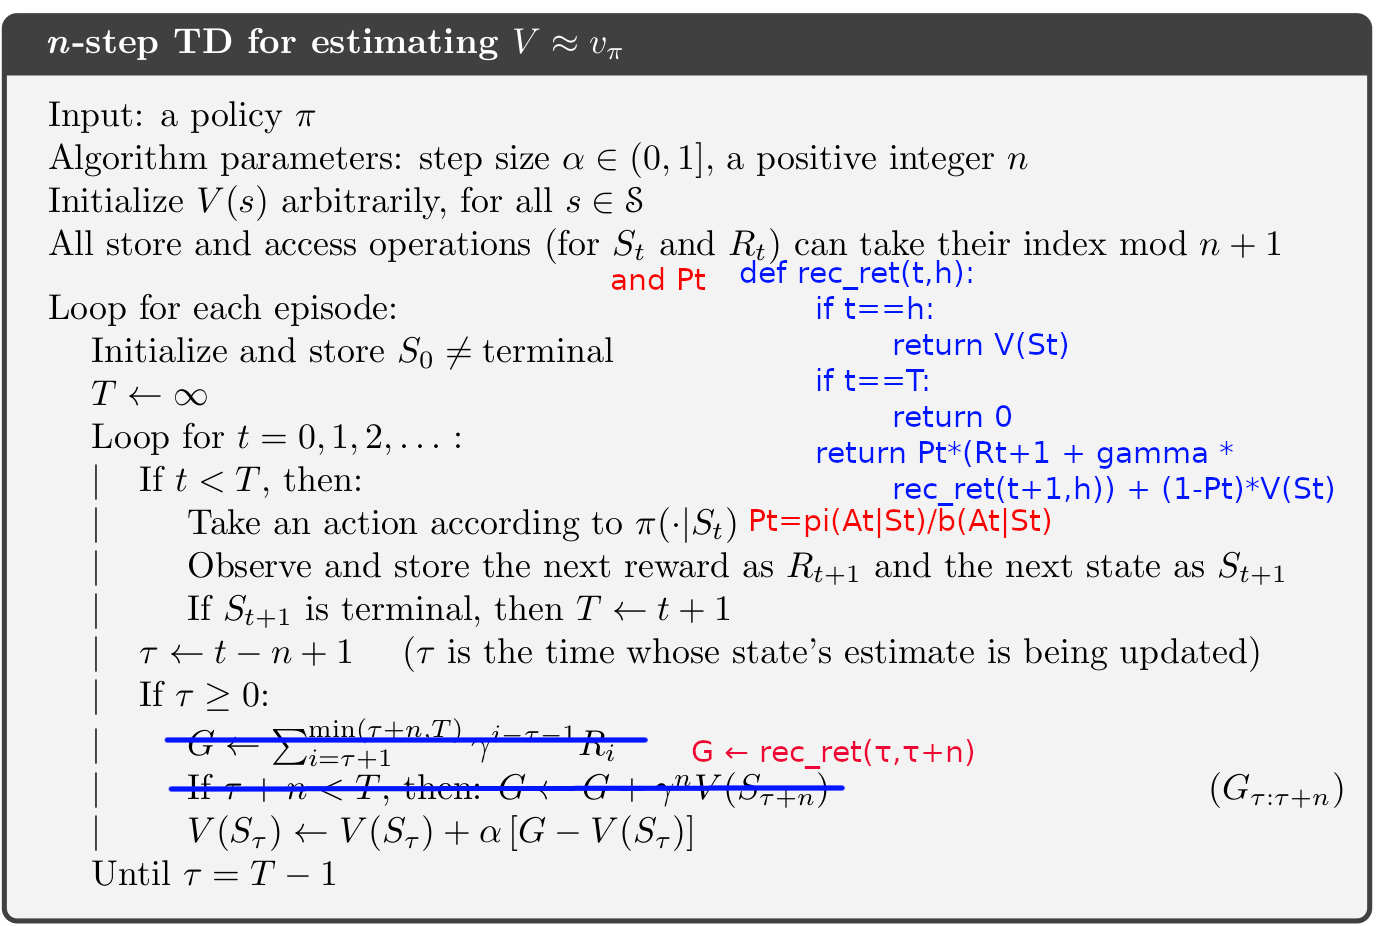
\includegraphics[scale=1]{figure_7_5}

    \subsection{Question}

    Prove that the control variate in the above equations does not change the expected value of the return.

    \subsection*{Answer}

    We have $ E[\rho_t] = E[\frac{\pi(A_t|S_t)}{b(A_t|S_t)}] = 1 $ from 5.13.

    \noindent Equation 7.14:

    \noindent $ G_{t:h} = R_{t+1} \gamma \rho_{t+1} ( G_{t+1:h} - Q_{h-1}(S_{t+1}, A_{t+1}) + \gamma \bar{V}_{h-1}(S_{t+1}) ) $

    \noindent The expected value is:

    \noindent $ E[G_{t:h}] = E [R_{t+1} + \gamma \rho_{t+1} ( G_{t+1:h} - Q_{h-1}(S_{t+1}, A_{t+1}) )+ \gamma \bar{V}_{h-1}(S_{t+1}) ] $

    \noindent Using Linearity of expectation and 5.13:

    \noindent $ E[G_{t:h}] = E [R_{t+1}] + \gamma E[( G_{t+1:h} - Q_{h-1}(S_{t+1}, A_{t+1}) )] + \gamma E[\bar{V}_{h-1}(S_{t+1})] $

    \noindent $ E[G_{t:h}] = E [R_{t+1}] + \gamma E[G_{t+1:h}] - \gamma E[Q_{h-1}(S_{t+1}, A_{t+1}) ] + \gamma E[\bar{V}_{h-1}(S_{t+1})] $

    \noindent Using 7.8:

    \noindent $ E[G_{t:h}] = E [R_{t+1}] + \gamma E[G_{t+1:h}] - \gamma E[\bar{V}_{h-1}(S_{t+1})] + \gamma E[\bar{V}_{h-1}(S_{t+1})] $

    \noindent $ E[G_{t:h}] = E [R_{t+1}] + \gamma E[G_{t+1:h}] $

    \noindent $ E[G_{t:h}] = E [R_{t+1} + \gamma G_{t+1:h}] $

    \noindent Using 7.12:

    \noindent $ E[G_{t:h}] = E[G_{t:h}] $


    \subsection{Question}

    Write the pseudocode for the off-policy action-value prediction algorithm described immediately above.

    \subsection*{Answer}

    The pseudo-code for "n-step sarsa for estimating" modified which reflects equation 7.11.

    Return is calculated as defined in equation 7.14.

    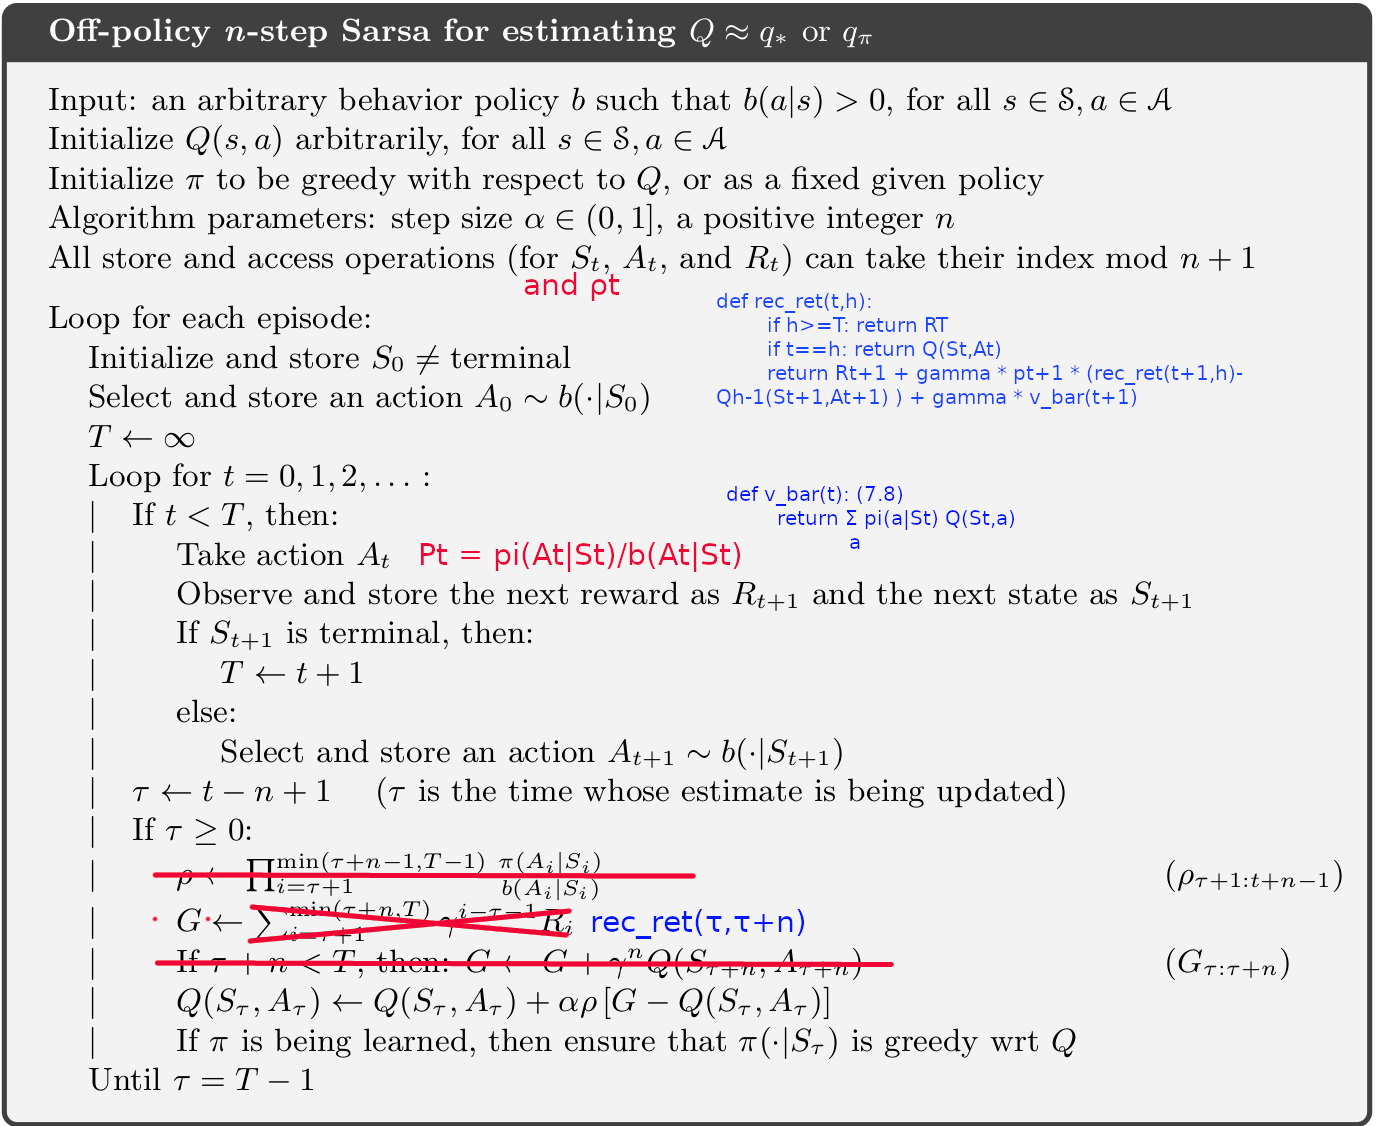
\includegraphics[scale=1]{figure_7_7}


    \subsection{Question}

    Show that the general (off-policy) version of the n-step return (7.13) can still be written exactly and compactly as the sum of state-based TD errors (6.5) if the  approximate state value function does not change.

    \subsection*{Answer}

    Equation 7.13:

    $ G_{t:h} =  \rho_t (R_{t+1} + \gamma G_{t+1:h} ) + (1 - \rho_t) V_{h-1}(S_t) $

    \noindent Assuming state value function does not change.

    \noindent $ G_{t:h} = \rho_t (R_{t+1} + \gamma G_{t+1:h} ) + (1 - \rho_t) V(S_t) $

    \noindent $ G_{t:h} = \rho_t (R_{t+1} + \gamma G_{t+1:h} - V(S_t)) + V(S_t)  $

    \noindent $ G_{t:h} = \rho_t (R_{t+1} + \gamma G_{t+1:h} - V(S_t) + \gamma V(S_{t+1}) - \gamma V(S_{t+1})) + V(S_t)  $

    \noindent $ G_{t:h} = \rho_t (R_{t+1} + \gamma V(S_{t+1})- V(S_t)  + \gamma G_{t+1:h} - \gamma V(S_{t+1})) + V(S_t)  $

    \noindent $ G_{t:h} = \rho_t (\delta_t  + \gamma G_{t+1:h} - \gamma V(S_{t+1})) + V(S_t)  $

    \noindent $ G_{t:h} = \rho_t (\delta_t  + \gamma (G_{t+1:h} - V(S_{t+1}) )) + V(S_t)  $

    \noindent $ G_{t:h} = \rho_t (\delta_t  + \gamma (   \rho_{t+1} (R_{t+2} + \gamma G_{t+2:h} - V(S_{t+1})) + V(S_{t+1})  - V(S_{t+1}) )) + V(S_t)  $

    \noindent $ G_{t:h} = \rho_t (\delta_t  + \gamma (   \rho_{t+1} (R_{t+2} + \gamma G_{t+2:h} - V(S_{t+1})) )) + V(S_t)  $

    \noindent $ G_{t:h} = \rho_t \delta_t  + \gamma \rho_{t:t+1} \delta_{t+1} + \dots + \gamma^{h-1} \rho_{t:h} (G_{h:h} - V(S_h)) + V(S_t)  $

    \noindent $ G_{t:h} = V(S_t) + \sum_{k=t}^{h-1}  \rho_{t:k} \gamma^{k-t} \delta_k  $

    \subsection{Question}

    Repeat the above exercise for the action version of the off-policy n-step return (7.14) and the Expected Sarsa TD error (the quantity in brackets in Equation 6.9).

    \subsection*{Answer}

    Expected Sarsa TD error (the quantity in brackets in Equation 6.9):

    \noindent $ \delta_{t} = R_{t+1} + \gamma \bar{V}(S_{t+1}) -Q(S_t,A_t) $

    \noindent Equation 7.14:

    \noindent $ G_{t:h} = R_{t+1} + \gamma \rho_{t+1} (G_{t+1:h} - Q(S_{t+1},A_{t+1} )) + \gamma \bar{V}(S_{t+1}) $

    \noindent $ G_{t:h} = R_{t+1} + \gamma \bar{V}(S_{t+1}) -Q(S_t,A_t) + \gamma \rho_{t+1} (G_{t+1:h} - Q(S_{t+1},A_{t+1} ))  + Q(S_t,A_t)  $

    \noindent $ G_{t:h} = \delta_{t} + \gamma \rho_{t+1} (G_{t+1:h} - Q(S_{t+1},A_{t+1} ))  + Q(S_t,A_t) $

    \noindent $ G_{t:h} = \delta_{t} + \gamma \rho_{t+1} ( [ R_{t+2} + \gamma \rho_{t+2} (G_{t+2:h} - Q(S_{t+2},A_{t+2} )) + \gamma \bar{V}(S_{t+2}) ] - Q(S_{t+1},A_{t+1} )) + Q(S_t,A_t)$

    \noindent $ G_{t:h} = \delta_{t} + \gamma \rho_{t+1} (  \delta_{t+1} + \gamma \rho_{t+2} (G_{t+2:h} - Q(S_{t+2},A_{t+2} )) + Q(S_{t+1},A_{t+1}) - Q(S_{t+1},A_{t+1}) ) + Q(S_t,A_t) $

    \noindent $ G_{t:h} = \delta_{t} + \gamma \rho_{t+1} (  \delta_{t+1} + \gamma \rho_{t+2} (G_{t+2:h} - Q(S_{t+2},A_{t+2} ))  ) + Q(S_t,A_t) $

    \noindent $ G_{t:h} = \delta_{t} + \gamma \rho_{t+1} \delta_{t+1} + \gamma^2 \rho_{t+1:t+2} ( G_{t+2:h} - Q(S_{t+2},A_{t+2} ))  + Q(S_t,A_t) $

    \noindent $ G_{t:h} = \delta_{t} + \gamma \rho_{t+1} \delta_{t+1} + \gamma^2 \rho_{t+1:t+2} ( \delta_{t+2} +  G_{t+3:h} - Q(S_{t+3},A_{t+3} )  )  + Q(S_t,A_t) $

    \noindent $ G_{t:h} = \delta_{t} + \gamma \rho_{t+1} \delta_{t+1} + \gamma^2 \rho_{t+1:t+2} \delta_{t+2} +  \gamma^2 \rho_{t+1:t+2} (G_{t+3:h} - Q(S_{t+3},A_{t+3} )  )   + Q(S_t,A_t) $

    \noindent $ G_{t:h} = \delta_{t} + \gamma \rho_{t+1} \delta_{t+1} + \gamma^2 \rho_{t+1:t+2} \delta_{t+2} + \dots + \gamma^{h-t-2} \rho_{t+1:h-2} \delta_{h-2} + \gamma^{h-t-1} \rho_{t+1:h-1} (G_{h:h} - Q(S_{h},A_{h} )  )  + Q(S_t,A_t) $

    \noindent since $ G_{h:h} = Q(S_h,A_h) $

    \noindent $ G_{t:h} = \delta_{t} + \gamma \rho_{t+1} \delta_{t+1} + \gamma^2 \rho_{t+1:t+2} \delta_{t+2} + \dots +  \gamma^{h-t-2} \rho_{t+1:h-2} \delta_{h-2} + Q(S_t,A_t) $

    \noindent $ G_{t:h} = Q(S_t,A_t) + \sum_{k=t}^{h-2} \gamma^{k-t} \rho_{t+1:k} \delta_k $ (given $ \rho_{t:h} = 1$ if $ t>h $ )


    \subsection{Question}

    (programming) Devise a small off-policy prediction problem and use it to show that the off-policy learning algorithm using (7.13) and (7.2) is more data efficient than the simpler algorithm using (7.1) and (7.9).

    \subsection*{Answer}

    Data efficiency is measured by looking at how fast state values converges.
    All state values are summed and averaged.
    The chart below shows average state value at episode for the simple and sophisticated approaches.

    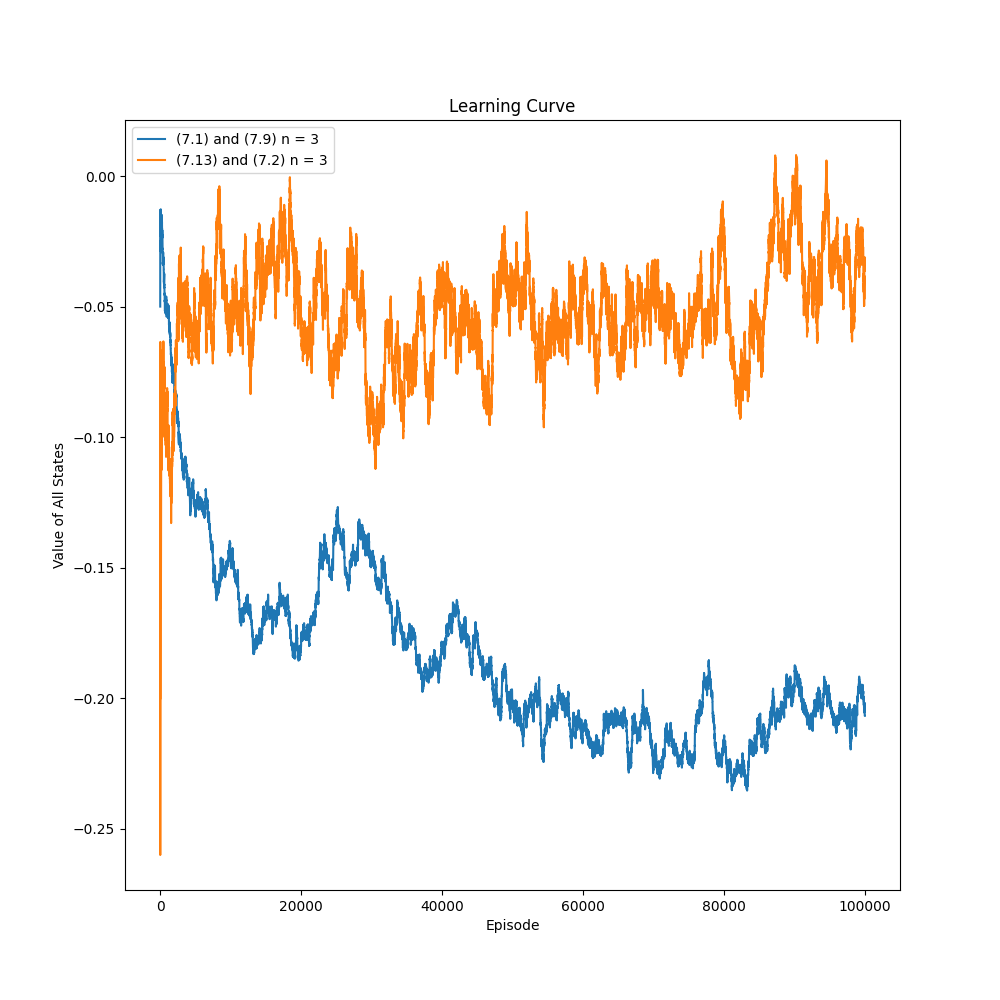
\includegraphics[scale=0.5]{figure_7_10}

    My experimental finding is that: The sophisticated approach suffers from the control variate.
    When an action is optimal and not favored by the random policy (e.g. $ \rho_t = 1.0/0.5 = 2 $), resulting importance sampling ratio signifies not only the return term but also the control variate.
    This makes the returns fluctuate.
    This may be due to an implementation or setup error.

    However, the simpler TD seems to work better thus more data efficient.

     \subsection{Question}

    Show that if the approximate action values are unchanging, then the tree-backup return (7.16) can be written as a sum of expectation-based TD errors:

    \subsection*{Answer}

    Equation 7.16:

    \noindent $ G_{t:t+n} = R_{t+1} + \gamma \sum_{a \neq A_{t+1}} \pi(a|S_{t+1}) Q_{t+n-1}(S_{t+1},a) + \gamma \pi(A_{t+1}|S_{t+1}) G_{t+1:t+n} $

    \noindent $ G_{t:t+n} = R_{t+1} + \gamma \bar{V}(S_{t+1}) - \gamma \pi(A_{t+1}|S_{t+1}) Q(S_{t+1},A_{t+1}) + \gamma \pi(A_{t+1}|S_{t+1}) G_{t+1:t+n} $

    \noindent $ G_{t:t+n} = R_{t+1} + \gamma \bar{V}(S_{t+1}) - Q(S_{t},A_{t}) + Q(S_{t},A_{t}) - \gamma \pi(A_{t+1}|S_{t+1}) Q(S_{t+1},A_{t+1}) + \gamma \pi(A_{t+1}|S_{t+1}) G_{t+1:t+n} $

    \noindent $ G_{t:t+n} = \delta_{t} + Q(S_{t},A_{t}) - \gamma \pi(A_{t+1}|S_{t+1}) Q(S_{t+1},A_{t+1}) + \gamma \pi(A_{t+1}|S_{t+1}) G_{t+1:t+n} $

    We will use the above form to replace future G values in subsequent equations.

    \noindent $ G_{t:t+n} = \delta_{t} + Q(S_{t},A_{t}) - \gamma \pi(A_{t+1}|S_{t+1}) Q(S_{t+1},A_{t+1}) + \gamma \pi(A_{t+1}|S_{t+1}) (\delta_{t+1} + Q(S_{t+1},A_{t+1}) - \gamma \pi(A_{t+2}|S_{t+2}) Q(S_{t+2},A_{t+2}) + \gamma \pi(A_{t+2}|S_{t+2}) G_{t+2:t+n}) $

    \noindent $ G_{t:t+n} = \delta_{t} + Q(S_{t},A_{t}) + \gamma \pi(A_{t+1}|S_{t+1}) (\delta_{t+1} - \gamma \pi(A_{t+2}|S_{t+2}) Q(S_{t+2},A_{t+2}) + \gamma \pi(A_{t+2}|S_{t+2}) G_{t+2:t+n})  $

    \noindent $ G_{t:t+n} = Q(S_{t},A_{t}) + \delta_{t} + \gamma \pi(A_{t+1}|S_{t+1}) \delta_{t+1} + \gamma \pi(A_{t+1}|S_{t+1}) (- \gamma \pi(A_{t+2}|S_{t+2}) Q(S_{t+2},A_{t+2}) + \gamma \pi(A_{t+2}|S_{t+2}) G_{t+2:t+n}) $

    \noindent $ G_{t:t+n} = Q(S_{t},A_{t}) + \delta_{t} + \gamma \pi(A_{t+1}|S_{t+1}) \delta_{t+1} - \gamma^2 \pi(A_{t+1}|S_{t+1}) \pi(A_{t+2}|S_{t+2}) Q(S_{t+2},A_{t+2}) + \gamma^2 \pi(A_{t+1}|S_{t+1}) \pi(A_{t+2}|S_{t+2}) G_{t+2:t+n} $

    Replace G one more time.

    \noindent $ G_{t:t+n} = Q(S_{t},A_{t}) + \delta_{t} + \gamma \pi(A_{t+1}|S_{t+1}) \delta_{t+1} - \gamma^2 \pi(A_{t+1}|S_{t+1}) \pi(A_{t+2}|S_{t+2}) Q(S_{t+2},A_{t+2}) + \gamma^2 \pi(A_{t+1}|S_{t+1}) \pi(A_{t+2}|S_{t+2}) [\delta_{t+2} + Q(S_{t+2},A_{t+2}) - \gamma \pi(A_{t+3}|S_{t+3}) Q(S_{t+3},A_{t+3}) + \gamma \pi(A_{t+3}|S_{t+3}) G_{t+3:t+n}] $

    \noindent $ G_{t:t+n} = Q(S_{t},A_{t}) + \delta_{t} + \gamma \pi(A_{t+1}|S_{t+1}) \delta_{t+1} + \gamma^2 \pi(A_{t+1}|S_{t+1}) \pi(A_{t+2}|S_{t+2}) [\delta_{t+2} - \gamma \pi(A_{t+3}|S_{t+3}) Q(S_{t+3},A_{t+3}) + \gamma \pi(A_{t+3}|S_{t+3}) G_{t+3:t+n}] $

    \noindent $ G_{t:t+n} = Q(S_{t},A_{t}) + \delta_{t} + \gamma \pi(A_{t+1}|S_{t+1}) \delta_{t+1} + \gamma^2 \pi(A_{t+1}|S_{t+1}) \pi(A_{t+2}|S_{t+2}) \delta_{t+2} + \gamma^2 \pi(A_{t+1}|S_{t+1}) \pi(A_{t+2}|S_{t+2}) [ - \gamma \pi(A_{t+3}|S_{t+3}) Q(S_{t+3},A_{t+3}) + \gamma \pi(A_{t+3}|S_{t+3}) G_{t+3:t+n}] $


        Equation 7.16:

    \noindent $ G_{t:t+n} = R_{t+1} + \gamma \sum_{a \neq A_{t+1}} \pi(a|S_{t+1}) Q_{t+n-1}(S_{t+1},a) + \gamma \pi(A_{t+1}|S_{t+1}) G_{t+1:t+n} $

    \noindent $ G_{t:t+n} = R_{t+1} + \gamma \bar{V}(S_{t+1}) - \gamma \pi(A_{t+1}|S_{t+1}) Q(S_{t+1},A_{t+1}) + \gamma \pi(A_{t+1}|S_{t+1}) G_{t+1:t+n} $

    \noindent $ G_{t:t+n} = R_{t+1} + \gamma \bar{V}(S_{t+1}) - Q(S_{t},A_{t}) + Q(S_{t},A_{t}) - \gamma \pi(A_{t+1}|S_{t+1}) Q(S_{t+1},A_{t+1}) + \gamma \pi(A_{t+1}|S_{t+1}) G_{t+1:t+n} $

    \noindent $ G_{t:t+n} = \delta_{t} + Q(S_{t},A_{t}) - \gamma \pi(A_{t+1}|S_{t+1}) Q(S_{t+1},A_{t+1}) + \gamma \pi(A_{t+1}|S_{t+1}) G_{t+1:t+n} $

    \noindent $ G_{t:t+n} = Q(S_{t},A_{t}) + \delta_{t} + \gamma \pi(A_{t+1}|S_{t+1})( G_{t+1:t+n} - Q(S_{t+1},A_{t+1})) $

    We will use the above form to replace future G values in subsequent equations.

    \noindent $ G_{t:t+n} = Q(S_{t},A_{t}) + \delta_{t} + \gamma \pi(A_{t+1}|S_{t+1})( \delta_{t+1} + Q(S_{t+1},A_{t+1}) + \gamma \pi(A_{t+2}|S_{t+2})( G_{t+2:t+n} - Q(S_{t+2},A_{t+2})) - Q(S_{t+1},A_{t+1}) ) $

    \noindent $ G_{t:t+n} = Q(S_{t},A_{t}) + \delta_{t} + \gamma \pi(A_{t+1}|S_{t+1})( \delta_{t+1} + \gamma \pi(A_{t+2}|S_{t+2})( G_{t+2:t+n} - Q(S_{t+2},A_{t+2})) ) $

    \noindent $ G_{t:t+n} = Q(S_{t},A_{t}) + \delta_{t} + \gamma \pi(A_{t+1}|S_{t+1}) \delta_{t+1} +\gamma^2 \pi(A_{t+1}|S_{t+1}) \pi(A_{t+2}|S_{t+2})( G_{t+2:t+n} - Q(S_{t+2},A_{t+2}))  $


    Replace G one more time.

    \noindent $ G_{t:t+n} = Q(S_{t},A_{t}) + \delta_{t} + \gamma \pi(A_{t+1}|S_{t+1}) \delta_{t+1} +\gamma^2 \pi(A_{t+1}|S_{t+1}) \pi(A_{t+2}|S_{t+2})( Q(S_{t+2},A_{t+2}) + \delta_{t+2} + \gamma \pi(A_{t+3}|S_{t+3})( G_{t+3:t+n} - Q(S_{t+3},A_{t+3})) - Q(S_{t+2},A_{t+2}))  $

    \noindent $ G_{t:t+n} = Q(S_{t},A_{t}) + \delta_{t} + \gamma \pi(A_{t+1}|S_{t+1}) \delta_{t+1} +\gamma^2 \pi(A_{t+1}|S_{t+1}) \pi(A_{t+2}|S_{t+2})( \delta_{t+2} + \gamma \pi(A_{t+3}|S_{t+3})( G_{t+3:t+n} - Q(S_{t+3},A_{t+3})))  $

    \noindent $ G_{t:t+n} = Q(S_{t},A_{t}) + \delta_{t} + \gamma \pi(A_{t+1}|S_{t+1}) \delta_{t+1} + \gamma^2 \pi(A_{t+1}|S_{t+1}) \pi(A_{t+2}|S_{t+2}) \delta_{t+2} + \gamma^3 \pi(A_{t+1}|S_{t+1}) \pi(A_{t+2}|S_{t+2}) \pi(A_{t+3}|S_{t+3})( G_{t+3:t+n} - Q(S_{t+3},A_{t+3}))  $

    G term will continue expanding at most n times until $ G_{t+n:t+n} $  where it will return $ Q(S_{t+n}, A_{t+n}) $ and last term cancels.
    If $ t=T-1$ it will return $R_t$ .

    Final recursive form will look like:

    \noindent $ G_{t:t+n} = Q(S_{t},A_{t}) + \sum_{i=t}^{\min(t+n,T-1)} \gamma^{i-t} \delta_{i} + \prod_{k=t+1}^{i} \pi(A_{k}|S_{k})   $



\end{document}


